\section{Introduction}

Here, we demonstrate the use of tags (evolvable labels that can be specified with imperfect matching) to identify memory positions in genetic programming (GP).
Specifically, we conducted a series of experiments using simple linear GP representations on five problems from the general program synthesis benchmark suite~\citep{helmuth_general_2015}.  
We show that tag-indexed memory does not substantively affect problem solving success relative to more traditional, direct-indexed memory.

In traditional software engineering, human programmers create variables with unique names to specify data that they are working with.  
These variables are inherently associated with locations in memory that are accessed by using the variable's name.
This technique for referencing values in memory is intentionally rigid, requiring programmers to precisely name the data they want to reference, and imprecision results in syntactic errors.
Many traditional GP systems that give genetic programs access to memory (\textit{e.g.}, indexable memory registers) use similarly rigid naming schemes where memory is numerically indexed, and mutation operators must guarantee the validity of memory-referencing instructions. 
Interestingly, although exact naming is the most intuitive referencing mechanism
for human programmers, evolution in other contexts (such as identifying modules to run~\citep{lalejini_what_2019}) has been shown to be more successful when program references are allowed to be inexact.
Beyond computer code, robustness to perturbations is also thought to be important in the evolution of complex biological systems~\citep{kitano_biological_2004}.

\begin{figure}
  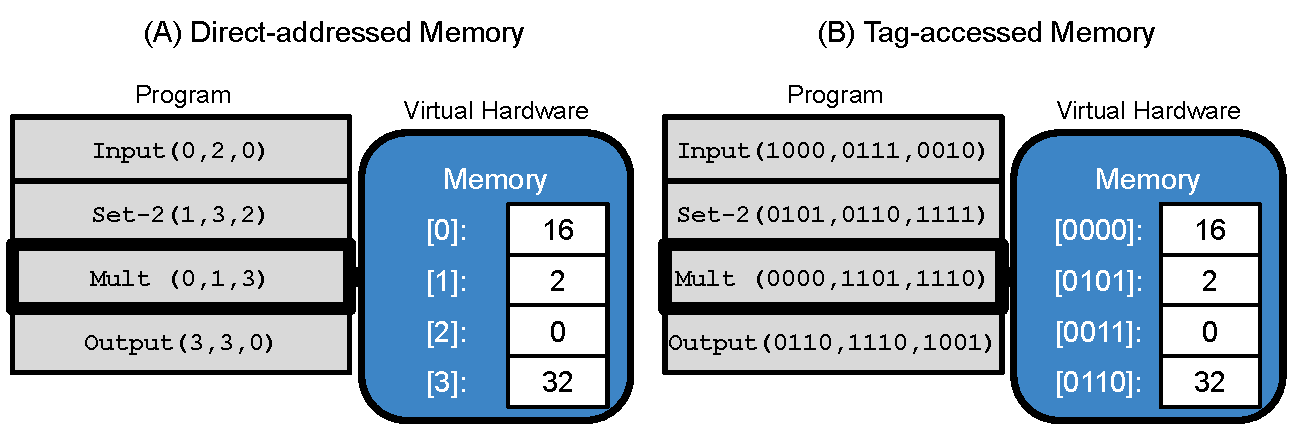
\includegraphics[width=1.0\columnwidth]{chapters/06-tag-access-memory/media/memory-access-overview.pdf}
  \caption{\small 
  Examples of (A) direct-indexed memory and (B) tag-accessed memory. 
  The programs in (A) and (B) behave identically: both request input to the first memory register, set the second memory register to the terminal value `2', place the result of multiplying the contents of the first two memory registers into the fourth memory register, and output the contents of the fourth register.
  Here, we show the state of memory after the \code{Mult} instruction has been executed. 
  Note that not all instructions use all three arguments.
  }
  \label{chapter:tag-accessed-memory:fig:memory-access-overview}
\end{figure}

% @AML: Here is where I describe tags and tag-based references.
Tags are evolvable labels that give genetic programs a flexible mechanism for specification, originally used by Holland in genetic algorithms \citep{holland_effect_1993} and refined by Spector \textit{et al.} for GP~\citep{spector_tag-based_2011}.
To facilitate \textit{inexact} referencing, the similarity (or dissimilarity) between any two tags must be quantifiable; a referring tag can always reference the closest matching referent tag.
Here, we continue to expand the integration of tags into linear GP by allowing instructions to use tags to identify positions in memory (as needed for their function).
All instructions have three tag-based arguments, each of which is represented as a length-16 bit string and compared using Hamming distance to measure similarity.
Our instruction set allows programs to perform basic computations, manipulate memory contents, and control execution flow (see supplemental material~\citep{tag_accessed_memory_supplement_2019} for details).
Programs are executed in the context of a virtual CPU that gives them access to 16 statically tagged memory registers used for storing data for performing computations.
Figure \ref{chapter:tag-accessed-memory:fig:memory-access-overview} contrasts tag-based memory with direct-indexed memory.
Tag-based instruction arguments reference the memory position with the \textit{closest matching} tag; as such, argument tags need not \textit{exactly} match any of the tags associated with memory positions.
This inexactness makes program phenotypes more robust to minor genetic perturbations, smoothing the genotype-phenotype mapping relative to more traditional memory-indexing techniques.
